%----------------------------------------
% Preamble to set up the document
%----------------------------------------
\documentclass{article}

% set up packages (you shouldn't need to touch this)
\usepackage{graphicx}  % required to insert images
\usepackage{hyperref}  % for hyperlinks
\usepackage[svgnames]{xcolor}  % to change hyperlink colors
\colorlet{linkcolour}{DarkBlue}
\hypersetup{colorlinks=true, linkcolor=linkcolour, citecolor=linkcolour, urlcolor=linkcolour,}

% Margins
\topmargin=-0.45in
\evensidemargin=0in
\oddsidemargin=0in
\textwidth=6.5in
\textheight=9.0in
\headsep=0.25in

% use a sans serif font
\renewcommand{\familydefault}{\sfdefault}

%----------------------------------------
% Step 1: Edit the lecture title
%----------------------------------------
\title{
Lecture 7: Regression, Part 2 \\  % Lecture title
Modeling Social Data, Spring 2017 \\   % Course title
Columbia University                    % School
}

%----------------------------------------
% Step 2: Edit your name and the date
%----------------------------------------
\author{Ingil Hwang}                     % Scribe's name
\date{March 3, 2017}                % Lecture date

\begin{document}

\maketitle


%----------------------------------------
% Step 3:
% Rename uni.tex to match your uni,
% edit the filename accordingly below,
% and put your notes in this file
%----------------------------------------
%----------------------------------------
% Write your notes here
%----------------------------------------
\section{From the Previous Lecture}

We have learned the general mathematical formulas and reasoning behind why we use linear regression for the presentation of the data. In many cases, linear regression can be a great tool in presenting the general trend of the data. 
Using the same data we used at the end of the last lecture, we can see that each dot on the graph is the average for a certain age group. By looking at these data points and the general trend curve, we can make a prediction(which in fact is our end goal in finding the "best" model). We can also manipulate data so that we can select specific data based on different category. After plotting predicted and actual data, we can use different colors to plot the trend curves by gender and age.

\section{Evaluating the fit of model}

One of the key information in the data we miss out with this trend curve is variation in the data. It might be the case that two different sets of data with almost identical trend curve have drastically different data. This can be due to the difference in the variability, which has the real world implication. So we need to take standard deviation into consideration when we evaluate the fit of model. There are two commonly used formula: root mean square error and Pearson's correlation coefficient.
\begin{itemize}
\item Root mean square error (RMSE)\[\sqrt{\frac{1}{N}\sum_{i}^{N}(y_i-\hat{y})^2}\]
The RMSD represents the sample standard deviation of the differences between predicted values and observed value. 
\item Pearson's correlation coefficient (PCC)\[\frac{\sum_i(y_i-\bar{y})(\hat{y_i}-\hat{\bar{y}})}{[\sum_i(y_i-\bar{y})^2]^\frac{1}{2}[\sum_i(\hat{y_i}-\hat{\bar{y}})^2]^\frac{1}{2}}\]
The PCC is a measure of the linear dependence (correlation) between two variables X and Y. In a nutshell, PCC is the covariance of the two variables divided by the product of their standard deviations. 
\end{itemize}

\section{Trade-off between Accuracy and Prediction}

When fitting a curve to the data, we often have to deal with a question of how much accurate do we want the function to be. While making the curve fit very accurately to the data can look good and seem to be a good representation, a too accurate model can perform badly in predicting future since it is overly sensitive to noise, which is the definition of "overfitting." On the other hand, we would not want our curve to be too loose to the extent that the given data does little in predicting future, "underfitting". This complexity is represented by the order of a function -- the higher it is, the more complex the model gets. 

\begin{figure}[ht]
  \begin{center}
    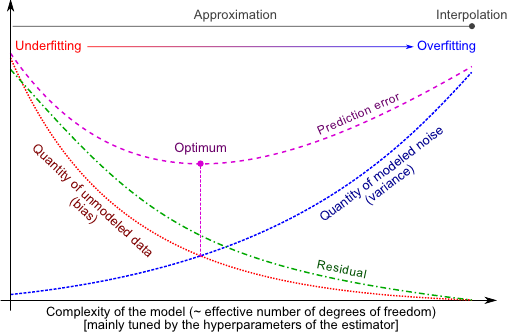
\includegraphics[width=0.5\textwidth]{figures/figure1.png}
    \caption{
      source: http://www.brnt.eu/phd/node14.html}
    \label{fig:example_figure}
  \end{center}
\end{figure}
As we can see from the above graph, the optimal point of accuracy happens somewhere in-between overfitting and underfitting.\newline 

\section{Bias- and Variance Trade-off}
\[MSE = Bias^2 + Variance + Irreducible Error\]

\begin{figure}[ht]
  \begin{center}
    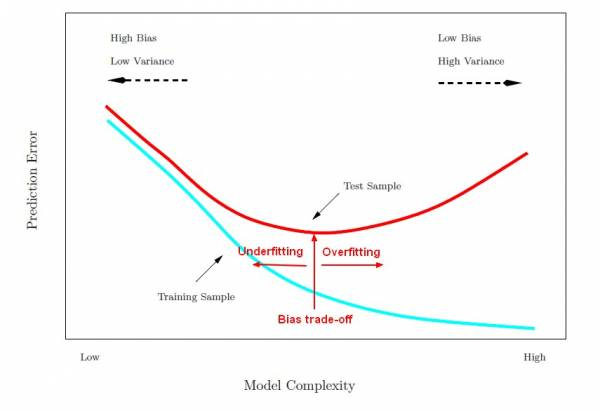
\includegraphics[width=0.5\textwidth]{figures/figure2.jpg}
    \caption{
      source: http://gerardnico.com/wiki/ }
    \label{fig:example_figure}
  \end{center}
\end{figure}
Low variance: It does not change a lot as it gets difficult.\newline High variance: Model changes a lot with different draws of the data. \newline
High Bias: Assumes something that might not be true, so it could always be wrong even with infinite amount of data\newline Low Bias: Can capture complicated patterns with enough data.

\section{Setting complexity}

So now we know choosing the right complexity, i.e. degree of functions is important. To evaluate this, we fit the models on the "training set", and test with "validation set". These two sets should be randomly chosen so that we can test the model.
\newline More generally, to find a good model 
\begin{itemize}
\item randomly split our data into 3 sets
\item fit models on the training set
\item Use the validation set to find the best model (different data)
\item Quote final performance of this model on the test set
\end{itemize}

One technique we can make a good use of is "K-fold cross validation." We take a subset of data as a validation data out of training data, and run the test. Then we take another subset out of the training data as a new validation data. Do this until every data has been used as a training data once. Finally, average all runs. Beware that we need to make sure the data is randomized. Then we can generate many test cases based on the real examples. We choose the order of the function that is minimum. It does not have to be strictly the minimum, however,  as it depends on each test. Rather, find the lowest order that is among the flat low line by looking at it.

\begin{figure}[ht]
  \begin{center}
    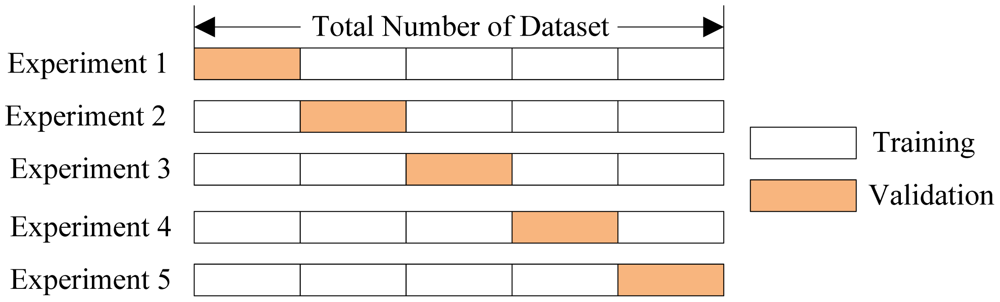
\includegraphics[width=0.5\textwidth]{figures/figure3.png}
    \caption{
      K-fold Cross Validation (source: http://sdsawtelle.github.io/blog/output/week6-andrew-ng-machine-learning-with-python.html)}
    \label{fig:example_figure}
  \end{center}
\end{figure}

Another technique is adding a random noise to the existing data and use that as training/validation data. The noise-generating technique is more advance and was briefly discussed during the lecture.

\section{Regularization}
Lastly, we discussed on ways to penalize complexity of the function.
\begin{itemize}
\item Ridge Regularization: \[\mathcal{L}=\frac{1}{n}\sum_i^n(y_i-wx_i)^2+\lambda \vert\vert w\vert\vert^2\]As \(\lambda\) increases, the coefficients decrease and reduces the weight of the model fit.
\item Lasso Regularization: \[\mathcal{L}=\frac{1}{n}\sum_i^n(y_i-wx_i)^2+\vert\vert w_1\vert\vert+\vert\vert w_2\vert\vert+...\] We can ignore near-zero coefficients.
\end{itemize}


\end{document}

%%% Local Variables:
%%% mode: latex
%%% TeX-master: t
%%% End:
